\documentclass[tikz]{standalone}

\usepackage{pgfplots}
\pgfplotsset{compat=newest}

\usepackage{tkz-tab}
\usepackage{amsmath}

\begin{document}

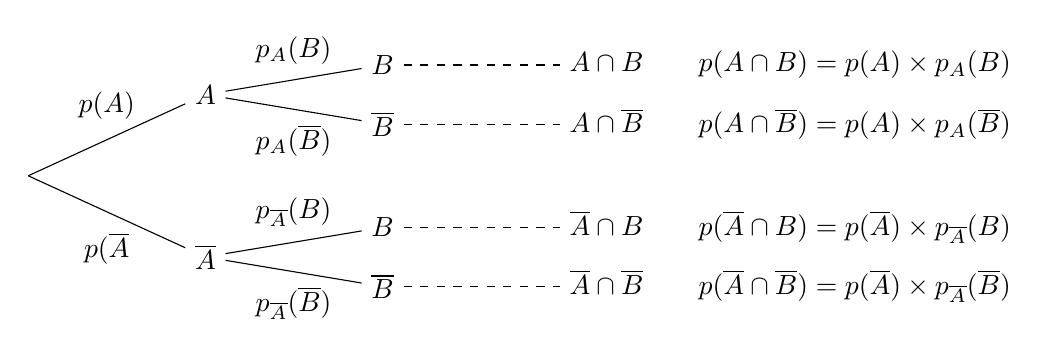
\begin{tikzpicture}[grow=right,level distance=3cm,scale=.75]
	\coordinate
		child[sibling distance=2.75cm] {
			node {$\overline{A}$}
			child[sibling distance=1cm] {
				node {$\overline{B}$}
				child{
					node[right] {
						$\overline{A}\cap\overline{B} \qquad p(\overline{A}\cap\overline{B})=p(\overline{A})\times p_{\overline{A}}(\overline{B})$}
					edge from parent[dashed]}
				edge from parent node[below=2pt] {$p_{\overline{A}}(\overline{B})$}}
			child[sibling distance=1cm] {
				node {$B$}
				child{
					node[right]{
						$\overline{A} \cap B\qquad p(\overline{A} \cap B)=p(\overline{A})\times p_{\overline{A}}(B)$}
					edge from parent[dashed]}
 				edge from parent node[above=2pt] {$p_{\overline{A}}(B)$}}
			edge from parent node[below=4pt] {$p(\overline{A}$}}
		child[sibling distance=2.75cm] {
			node {$A$}
 			child[sibling distance=1cm] {
				node {$\overline{B}$}
				child {
					node[right]{
						$A\cap\overline{B}\qquad p(A\cap\overline{B})=p(A)\times p_{A}(\overline{B})$}
					edge from parent[dashed]}
				edge from parent node[below=2pt] {$p_A(\overline{B})$}}
			child[sibling distance=1cm] {
				node {$B$}
				child{
					node[right]{
						$A\cap B\qquad p(A\cap B)=p(A)\times p_A(B)$}
					edge from parent[dashed]}
				edge from parent node[above=2pt] {$p_A(B)$}}
			edge from parent node[above=4pt] {$p(A)$}};
\end{tikzpicture}

\end{document}